\documentclass[11pt,a4paper]{article}

% Pakiety
\usepackage{iftex}
\ifXeTeX
  \usepackage{fontspec} % XeTeX/Tectonic: czcionki Unicode (domyślnie Latin Modern)
\else
  \usepackage[utf8]{inputenc}
  \usepackage[T1]{fontenc}
  \usepackage{lmodern}
\fi
\usepackage[polish]{babel}
\usepackage{xcolor}
\usepackage[a4paper,margin=2.1cm,headheight=14pt]{geometry}
\usepackage{amsmath,amssymb,amsthm,mathtools}
\usepackage{graphicx}
\usepackage{booktabs}
\usepackage{listings}
\usepackage{float}
\usepackage{algorithm}
\usepackage[noEnd=true]{algpseudocodex}
\usepackage[font=small,labelfont=normal]{caption}
\usepackage{fancyhdr}
\usepackage{titlesec}
\usepackage{microtype}

% Układ strony: nagłówek po prawej, numer strony na dole
\pagestyle{fancy}
\fancyhf{}
\fancyhead[R]{\small Hierarchiczna kompresja bitmapy z częściowym SVD}
\fancyfoot[C]{\thepage}
\renewcommand{\headrulewidth}{0pt}
\fancypagestyle{plain}{\fancyhf{}\fancyfoot[C]{\thepage}\renewcommand{\headrulewidth}{0pt}}

% Akapity i nagłówki sekcji (pogrubione, bezszeryfowe)
\setlength{\parindent}{1.5em}
\setlength{\parskip}{2pt}
\titleformat{\section}{\Large\bfseries\sffamily}{\thesection}{1em}{}
\titleformat{\subsection}{\large\bfseries\sffamily}{\thesubsection}{1em}{}
\titlespacing*{\section}{0pt}{12pt}{6pt}
\titlespacing*{\subsection}{0pt}{9pt}{4pt}
\renewcommand{\arraystretch}{1.1}

% Styl fragmentów kodu C++
\lstset{
  language=C++,
  basicstyle=\ttfamily\scriptsize,
  keywordstyle=\bfseries,
  commentstyle=\itshape\color[gray]{0.35},
  numbers=left, numberstyle=\tiny, numbersep=4pt,
  frame=single, framerule=0.3pt, rulecolor=\color[gray]{0.6},
  xleftmargin=10pt, aboveskip=3pt, belowskip=3pt,
  columns=fullflexible, keepspaces=true, showstringspaces=false
}

% Pseudokod: polskie słowa kluczowe
\floatname{algorithm}{Algorytm}
\algrenewcommand\algorithmicprocedure{\textbf{Procedura}}
\algrenewcommand\algorithmicif{\textbf{Jeżeli}}
\algrenewcommand\algorithmicthen{\textbf{wykonaj}}
\algrenewcommand\algorithmicelse{\textbf{W przeciwnym razie}}
\algrenewcommand\algorithmicreturn{\textbf{Zwróć}}
\algrenewcommand\algorithmicfor{\textbf{Dla}}
\algrenewcommand\algorithmicdo{\textbf{wykonaj}}

\newcommand{\CreateTree}{\textsc{CreateTree}}
\newcommand{\Compress}{\textsc{CompressMatrix}}

\begin{document}

\begin{center}
{\Large\bfseries\sffamily Hierarchiczna kompresja bitmapy z częściowym SVD}\\[0.6em]
Mateusz Majta, Maksymilian Siemek \quad|\quad Algorytmy Macierzowe 2026/2027, grupa 2
\end{center}

\section{Wstęp}
Zaimplementowaliśmy rekurencyjną (hierarchiczną) kompresję macierzy z wykorzystaniem częściowego rozkładu na
wartości osobliwe (SVD) z parametrami $r$ (maksymalny rząd bloku) i $\delta$ (próg: odrzucamy wartości osobliwe
mniejsze od $\delta$), rysowacz skompresowanej macierzy oraz rysowacz skompresowanej bitmapy. Jako bitmapę wybraliśmy
kolorowe zdjęcie Grace Hopper (domena publiczna, US Navy), przycięte do rozmiaru $512\times512$. Bitmapę zamieniamy
na trzy macierze R, G, B o wartościach z przedziału $[0,255]$ i każdą kompresujemy osobno.

\section{Język i sprzęt}
Algorytmy zaimplementowano w C++17. C++ nie jest językiem interpretowanym: kompilator (\texttt{g++}) zamienia cały
program z góry na kod maszynowy procesora, więc obliczenia nie przechodzą przez warstwę interpretera. Eksperymenty
wykonano na komputerze z procesorem AMD Ryzen 7 7735HS (8 rdzeni, 16 wątków), 32~GB pamięci RAM, systemem Windows~11,
kompilatorem \texttt{g++} 14.2.0 (MinGW-W64) z flagami \texttt{-O2 -std=c++17}. Trzy kanały R, G, B są kompresowane
równolegle w trzech wątkach. Bitmapy wejściowe i wyjściowe zapisujemy w najprostszym formacie PPM (nagłówek i bajty
R, G, B kolejnych pikseli); na potrzeby sprawozdania zamieniamy je na PNG.

\section{Algorytm}
\subsection{Częściowe SVD}
Każdy węzeł drzewa potrzebuje $r+1$ największych wartości osobliwych bloku oraz odpowiadających im wektorów:
$A\approx U\,\mathrm{diag}(\sigma_1,\dots,\sigma_{r+1})\,V^T$. Liczymy je jednostronną metodą Jacobiego (Hestenesa):
obracamy pary kolumn macierzy tak długo, aż wszystkie kolumny są do siebie prostopadłe. Wtedy długości kolumn są
wartościami osobliwymi, znormalizowane kolumny tworzą $U$, a złożenie obrotów daje $V$. Z wyniku zostawiamy $r+1$
największych wartości (częściowe SVD). Metoda jest prosta i dokładna także dla małych wartości osobliwych: dla
całych macierzy $512\times512$ wartości osobliwe zgadzają się z biblioteką \texttt{numpy} z błędem względnym
$10^{-10}$, a SVD trzech kanałów trwa 2{,}5\,s.

\subsection{Rekurencyjna kompresja}
Drzewo budujemy zgodnie z wykładem. Dla bloku liczymy częściowe SVD rzędu $r+1$. Jeśli $\sigma_{r+1}<\delta$, blok
jest dopuszczalny: zastępujemy go przybliżeniem rzędu $r$ (liść). W przeciwnym razie dzielimy go na cztery ćwiartki
i powtarzamy procedurę dla każdej z nich. Liść rzędu $k$ dla bloku $a\times b$ przechowuje $U$ ($a\times k$) oraz
$V=D\,V^T$ ($k\times b$), czyli $k(a+b)$ liczb zamiast $ab$. Blok zerowy jest liściem rzędu 0, a w liściu pomijamy
zerowe wartości osobliwe (np.\ blok $1\times1$ ma tylko jedną).

\begin{algorithm}[H]
\caption{Rekurencyjna kompresja macierzy}
\begin{algorithmic}[1]
\Procedure{\CreateTree}{$t_{\min},t_{\max},s_{\min},s_{\max},r,\delta$}
  \Comment{zakres wierszy i kolumn bloku macierzy $A$}
  \State $[U,D,V]\gets\textsc{truncatedSVD}(A(t_{\min}{:}t_{\max},\,s_{\min}{:}s_{\max}),\,r+1)$
  \If{$D(r{+}1,r{+}1)<\delta$ lub blok ma rozmiar $1\times1$}
    \State \Return $\Compress(t_{\min},t_{\max},s_{\min},s_{\max},U,D,V,r)$
  \EndIf
  \State utwórz węzeł $v$; $t_{\mathrm{new}}\gets\lfloor(t_{\min}+t_{\max})/2\rfloor$,
         $s_{\mathrm{new}}\gets\lfloor(s_{\min}+s_{\max})/2\rfloor$
  \State dodaj do $v$ syna $\CreateTree(t_{\min},t_{\mathrm{new}},s_{\min},s_{\mathrm{new}},r,\delta)$
  \State dodaj do $v$ syna $\CreateTree(t_{\min},t_{\mathrm{new}},s_{\mathrm{new}}{+}1,s_{\max},r,\delta)$
  \State dodaj do $v$ syna $\CreateTree(t_{\mathrm{new}}{+}1,t_{\max},s_{\min},s_{\mathrm{new}},r,\delta)$
  \State dodaj do $v$ syna $\CreateTree(t_{\mathrm{new}}{+}1,t_{\max},s_{\mathrm{new}}{+}1,s_{\max},r,\delta)$
  \State \Return $v$
\EndProcedure
\Statex
\Procedure{\Compress}{$t_{\min},t_{\max},s_{\min},s_{\max},U,D,V,r$}
  \If{blok składa się z zer}
    \State \Return liść $v$ z $v.\mathit{rank}=0$
  \EndIf
  \State $k\gets$ liczba niezerowych wartości wśród $D(1,1),\dots,D(r,r)$
  \State utwórz liść $v$; $v.\mathit{rank}\gets k$, $v.\sigma\gets\mathrm{diag}(D)(1{:}k)$
  \State $v.U\gets U(\ast,1{:}k)$, \quad $v.V\gets D(1{:}k,1{:}k)\cdot V(1{:}k,\ast)$
  \State \Return $v$
\EndProcedure
\end{algorithmic}
\end{algorithm}

\subsection{Rysowacze}
\emph{Rysowacz skompresowanej macierzy} tworzy obraz o rozmiarze macierzy. Każdy liść jest prostokątem z szarą
ramką. Liść rzędu $k$ ma czarny pasek szerokości $k$ wzdłuż lewej krawędzi (kolumny $U$) i czarny pasek wysokości $k$
wzdłuż górnej krawędzi (wiersze $V$). Czarne pole na rysunku odpowiada więc pamięci zajmowanej przez liść: duży
liść niskiego rzędu jest prawie biały, a liście $1\times1$ są całkowicie czarne.

\emph{Rysowacz skompresowanej bitmapy} odtwarza każdą macierz z drzewa (w każdym liściu blok $=U\cdot V$), przycina
wartości do $[0,255]$, zaokrągla do bajtów i składa kanały R, G, B w kolorową bitmapę. Pojedynczy kanał rysujemy
w jego kolorze (np.\ R jako odcienie czerwieni).

Jakość mierzymy błędem względnym $\|A-\tilde A\|_F/\|A\|_F$ każdego kanału i PSNR całej bitmapy,
$10\log_{10}(255^2/\mathrm{MSE})$. Pamięć podajemy jako liczbę przechowywanych liczb w stosunku do liczby pikseli
(100\% oznacza tyle liczb, ile wartości ma macierz).

\subsection{Najważniejsze fragmenty kodu}
\begin{figure}[H]
\centering
\begin{lstlisting}
std::unique_ptr<Node> createTree(const Matrix& A, int t0, int t1, int s0, int s1, int r, double eps) {
    Matrix block = subMatrix(A, t0, t1, s0, s1);
    if (isZero(block)) {                       // blok zerowy: lisc rzedu 0
        auto v = std::make_unique<Node>();
        v->t0 = t0, v->t1 = t1, v->s0 = s0, v->s1 = s1;
        return v;
    }
    SVD svd = truncatedSVD(block, r + 1);
    const bool single = (t1 - t0 == 1 && s1 - s0 == 1);  // bloku 1 x 1 nie da sie podzielic
    if (svd.sigma[r] < eps || single) return compressMatrix(t0, t1, s0, s1, svd, r);

    auto v = std::make_unique<Node>();
    v->t0 = t0, v->t1 = t1, v->s0 = s0, v->s1 = s1;
    const int tm = t0 + (t1 - t0 + 1) / 2, sm = s0 + (s1 - s0 + 1) / 2;
    const int rows[3] = {t0, tm, t1}, cols[3] = {s0, sm, s1};
    for (int a = 0; a < 2; ++a)
        for (int b = 0; b < 2; ++b)
            if (rows[a] < rows[a + 1] && cols[b] < cols[b + 1])  // pomijamy puste cwiartki
                v->sons.push_back(createTree(A, rows[a], rows[a + 1], cols[b], cols[b + 1], r, eps));
    return v;
}
\end{lstlisting}
\caption{Rekurencyjna kompresja (przedziały indeksów półotwarte: wiersze $[t_0,t_1)$, kolumny $[s_0,s_1)$).}
\end{figure}

\begin{figure}[H]
\centering
\begin{lstlisting}
std::unique_ptr<Node> compressMatrix(int t0, int t1, int s0, int s1, const SVD& svd, int r) {
    auto v = std::make_unique<Node>();
    v->t0 = t0, v->t1 = t1, v->s0 = s0, v->s1 = s1;
    int rank = 0;                              // rzad r bez zerowych wartosci osobliwych
    while (rank < r && svd.sigma[rank] > 1e-9 * svd.sigma[0]) ++rank;
    v->rank = rank;
    v->sigma.assign(svd.sigma.begin(), svd.sigma.begin() + rank);
    v->U = Matrix(t1 - t0, rank);
    v->V = Matrix(rank, s1 - s0);
    for (int k = 0; k < rank; ++k) {
        for (int i = 0; i < t1 - t0; ++i) v->U(i, k) = svd.U(i, k);
        for (int j = 0; j < s1 - s0; ++j) v->V(k, j) = svd.sigma[k] * svd.V(j, k);   // D * V^T
    }
    return v;
}

void drawNode(const Node& v, Image& img) {     // rysowacz skompresowanej macierzy
    if (!v.leaf()) { for (const auto& s : v.sons) drawNode(*s, img); return; }
    for (int j = v.s0; j < v.s1; ++j) paint(img, v.t0, j, 170);  // szara ramka
    for (int i = v.t0; i < v.t1; ++i) paint(img, i, v.s0, 170);
    for (int i = v.t0; i < v.t1; ++i)
        for (int j = v.s0; j < v.s1; ++j)
            if (i - v.t0 < v.rank || j - v.s0 < v.rank) paint(img, i, j, 0);   // paski U i V
}
\end{lstlisting}
\caption{Kompresja bloku i rysowacz skompresowanej macierzy.}
\end{figure}

\subsection{Sprawdzenie na przykładzie z wykładu}
Macierz z wykładu
$A=\left(\begin{smallmatrix}9&9&9&9\\2&6&10&14\\11&15&19&23\\32&33&34&35\end{smallmatrix}\right)$ ma rząd 2.
Program wyznacza jej wartości osobliwe $79{,}267$, $10{,}332$ oraz dwie rzędu $10^{-15}$. Dla $r=2$ i $\delta=10^{-6}$
korzeń jest od razu liściem rzędu 2: $16$ liczb (tyle co macierz), a $\max|A-\tilde A|=1{,}4\cdot10^{-14}$. Dla
$r=1$ żaden blok większy niż $1\times1$ nie ma rzędu 1 (np.\ $\left(\begin{smallmatrix}9&9\\2&6\end{smallmatrix}\right)$
ma rząd 2), więc drzewo schodzi do 16 liści $1\times1$, czyli 32 liczb. Kompresja jest bezstratna w obu
przypadkach, ale opłaca się tylko wtedy, gdy rząd bloków jest mały względem ich rozmiaru.

\section{Wartości osobliwe całej bitmapy}
\begin{figure}[H]
\centering
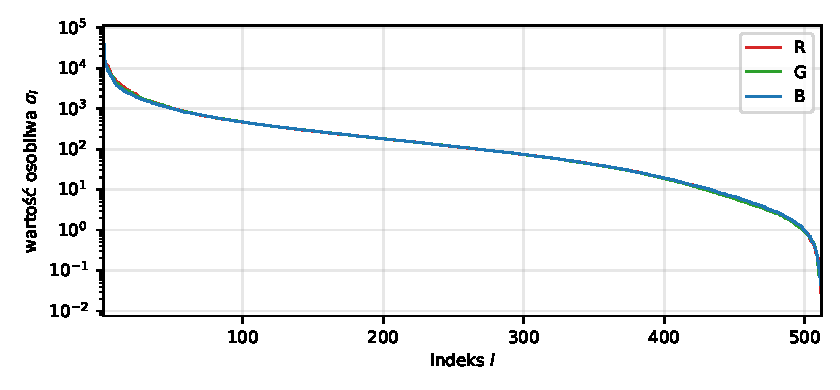
\includegraphics[width=0.72\textwidth]{fig/singular_values.pdf}
\caption{Wartości osobliwe $\sigma_1\ge\dots\ge\sigma_{512}$ całych macierzy R, G, B (skala logarytmiczna).}
\label{fig:sv}
\end{figure}

Macierze mają rozmiar $2^k\times2^k=512\times512$ ($k=9$), więc każda ma $2^k=512$ wartości osobliwych:
$\sigma_{2^k}=\sigma_{512}$ jest najmniejszą z nich, a $\sigma_{2^k/2}=\sigma_{256}$ środkową. Największe wartości to
$\sigma_1=53\,675$ (R), $45\,244$ (G), $53\,986$ (B); drugie są już około 4 razy mniejsze ($\sigma_2\approx13\,000$),
$\sigma_{100}\approx470$, środkowe $\sigma_{256}=110{,}9$ (R), $110{,}3$ (G), $111{,}7$ (B), $\sigma_{400}\approx19$,
a najmniejsze $\sigma_{512}=0{,}016$ (R), $0{,}042$ (G) i $0{,}036$ (B). Wartości maleją o sześć rzędów wielkości, ale
stopniowo, bez wyraźnego progu: zdjęcie nie ma małego rzędu i dobra kompresja wymaga podziału na bloki.

\section{Bitmapa nieskompresowana}
\begin{figure}[H]
\centering
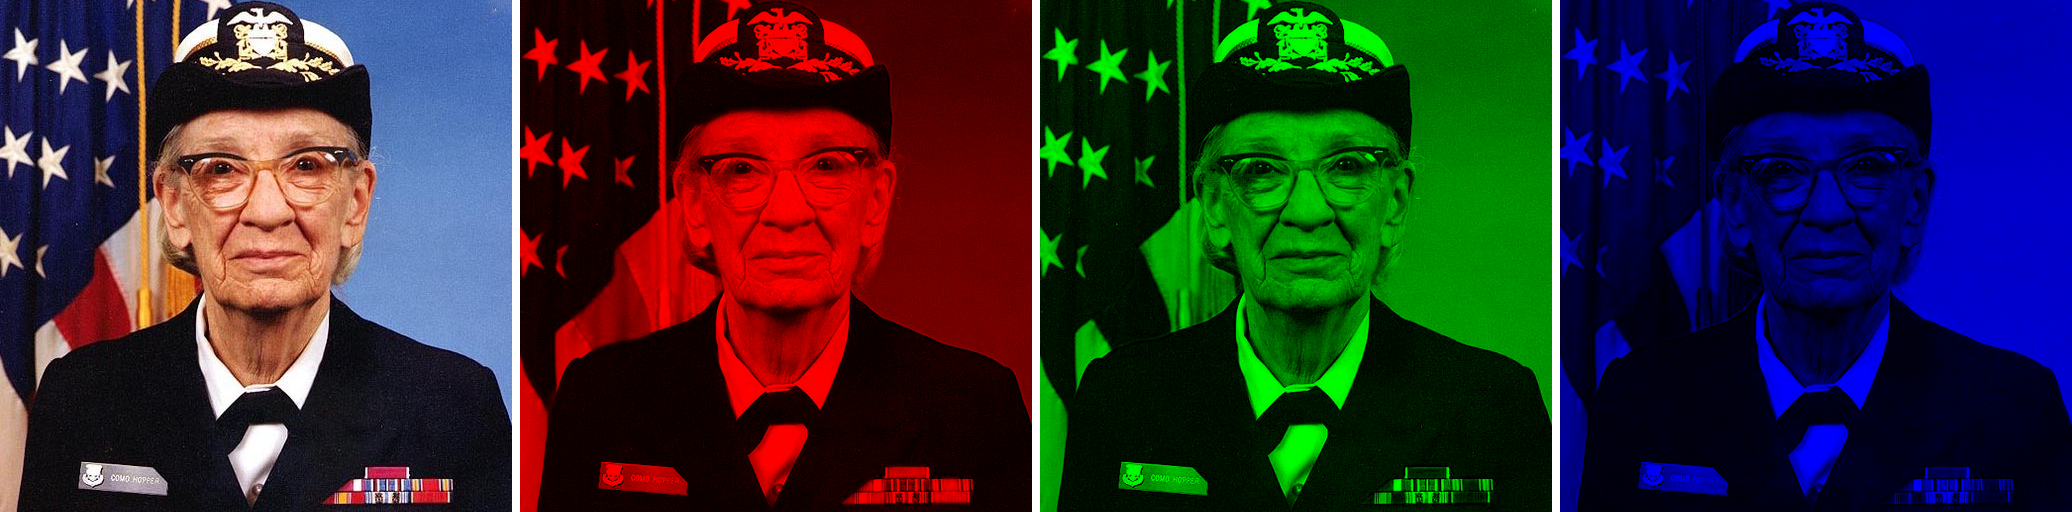
\includegraphics[width=\textwidth]{fig/oryginal.png}
\caption{Bitmapa $512\times512$: cała oraz osobno kanały R, G i B.}
\label{fig:oryginal}
\end{figure}

\section{Wyniki kompresji}
Na rysunkach~\ref{fig:r1s1}--\ref{fig:r4shalf} górny rząd to skompresowane macierze R, G, B (rysowacz macierzy),
dolny rząd to skompresowane kanały R, G, B, a po prawej jest wynikowa bitmapa RGB. Próg $\delta$ jest wyznaczany
osobno dla każdego kanału z jego wartości osobliwych. Tabela~\ref{tab:wyniki} zbiera liczby dla wszystkich
konfiguracji (liście i pamięć zsumowane po trzech kanałach).

\begin{table}[H]
\centering
\begin{tabular}{@{}lrrrrr@{}}
\toprule
konfiguracja & liście & głębokość & pamięć & maks.\ błąd względny & PSNR [dB]\\
\midrule
$r=1$, $\delta=\sigma_1$          & 3        & 0 & 0{,}39\%  & $5{,}4\cdot10^{-1}$  & 12{,}9\\
$r=1$, $\delta=\sigma_{2^k}$      & 750\,741 & 9 & 193{,}5\% & $1{,}9\cdot10^{-5}$  & $\infty$\\
$r=1$, $\delta=\sigma_{2^k/2}$    & 12\,456  & 8 & 18{,}5\%  & $7{,}1\cdot10^{-2}$  & 30{,}6\\
$r=4$, $\delta=\sigma_1$          & 3        & 0 & 1{,}56\%  & $3{,}9\cdot10^{-1}$  & 15{,}8\\
$r=4$, $\delta=\sigma_{2^k}$      & 49\,086  & 7 & 198{,}4\% & $5{,}8\cdot10^{-16}$ & $\infty$\\
$r=4$, $\delta=\sigma_{2^k/2}$    & 2\,331   & 7 & 36{,}4\%  & $4{,}2\cdot10^{-2}$  & 35{,}3\\
\midrule
$r=1$, $\delta=50$ (najlepsza)    & 27\,366  & 9 & 28{,}5\%  & $4{,}9\cdot10^{-2}$  & 33{,}9\\
\bottomrule
\end{tabular}
\caption{Wyniki kompresji (błąd względny: największy z kanałów R, G, B). PSNR $=\infty$ oznacza, że po zaokrągleniu do bajtów bitmapa jest identyczna z oryginałem.}
\label{tab:wyniki}
\end{table}

\paragraph{$\delta=\sigma_1$.} Druga wartość osobliwa całej macierzy jest mniejsza od pierwszej, więc już korzeń
spełnia warunek $\sigma_{r+1}<\sigma_1$ i cała macierz staje się jednym liściem rzędu $r$. Rysunek macierzy to jeden
prostokąt z cienkim paskiem szerokości $r$ (prawie biały). Pamięć jest minimalna ($r\cdot1024$ liczb na kanał), ale
bitmapa jest mocno rozmyta i ma pasy wzdłuż wierszy i kolumn, typowe dla przybliżenia niskiego rzędu. Kanały są
przybliżane niezależnie, więc w bitmapie RGB pojawiają się też fałszywe kolory.

\paragraph{$\delta=\sigma_{2^k}$ (najmniejsza wartość osobliwa).} Próg rzędu $10^{-2}$ jest tak mały, że blok jest
dopuszczalny tylko wtedy, gdy ma rząd co najwyżej $r$ (w granicach błędu zaokrągleń). Dla $r=1$ są to głównie bloki
$1\times1$: drzewo ma głębokość 9 i około 250 tysięcy liści na kanał, rysunek macierzy jest prawie cały czarny, a każdy
piksel zajmuje 2 liczby ($u$ i $v$), stąd pamięć około 194\%. Dla $r=4$ każdy blok $4\times4$ ma rząd co najwyżej 4,
więc $\sigma_5=0<\delta$ i drzewo kończy się na blokach $4\times4$ (głębokość 7, $4\cdot(4+4)=32$ liczby na 16
pikseli, czyli 198\%). Bitmapa jest odtworzona bezstratnie, ale drzewo zajmuje prawie dwa razy więcej miejsca niż
macierz.

\paragraph{$\delta=\sigma_{2^k/2}$ (środkowa wartość osobliwa).} Próg $\sigma_{256}\approx111$ daje kompresję
pośrednią. Blok jest dzielony tylko tam, gdzie jego $(r{+}1)$-sza wartość osobliwa przekracza około 111, czyli przy
krawędziach i drobnych szczegółach; gładkie obszary (tło, mundur) zostają dużymi liśćmi. Dla $r=1$ drzewo zajmuje
18{,}5\% pamięci przy PSNR 30{,}6\,dB: obraz jest czytelny, ale na tle i przy drobnych szczegółach widać lekkie rozmycie i granice bloków. Dla $r=4$
liście są większe i jest ich mniej (2\,331 zamiast 12\,456), każdy przechowuje jednak 4 razy więcej liczb, więc
pamięć rośnie do 36{,}4\%, a PSNR do 35{,}3\,dB i bitmapa jest prawie nieodróżnialna od oryginału.

\begin{figure}[H]
\centering
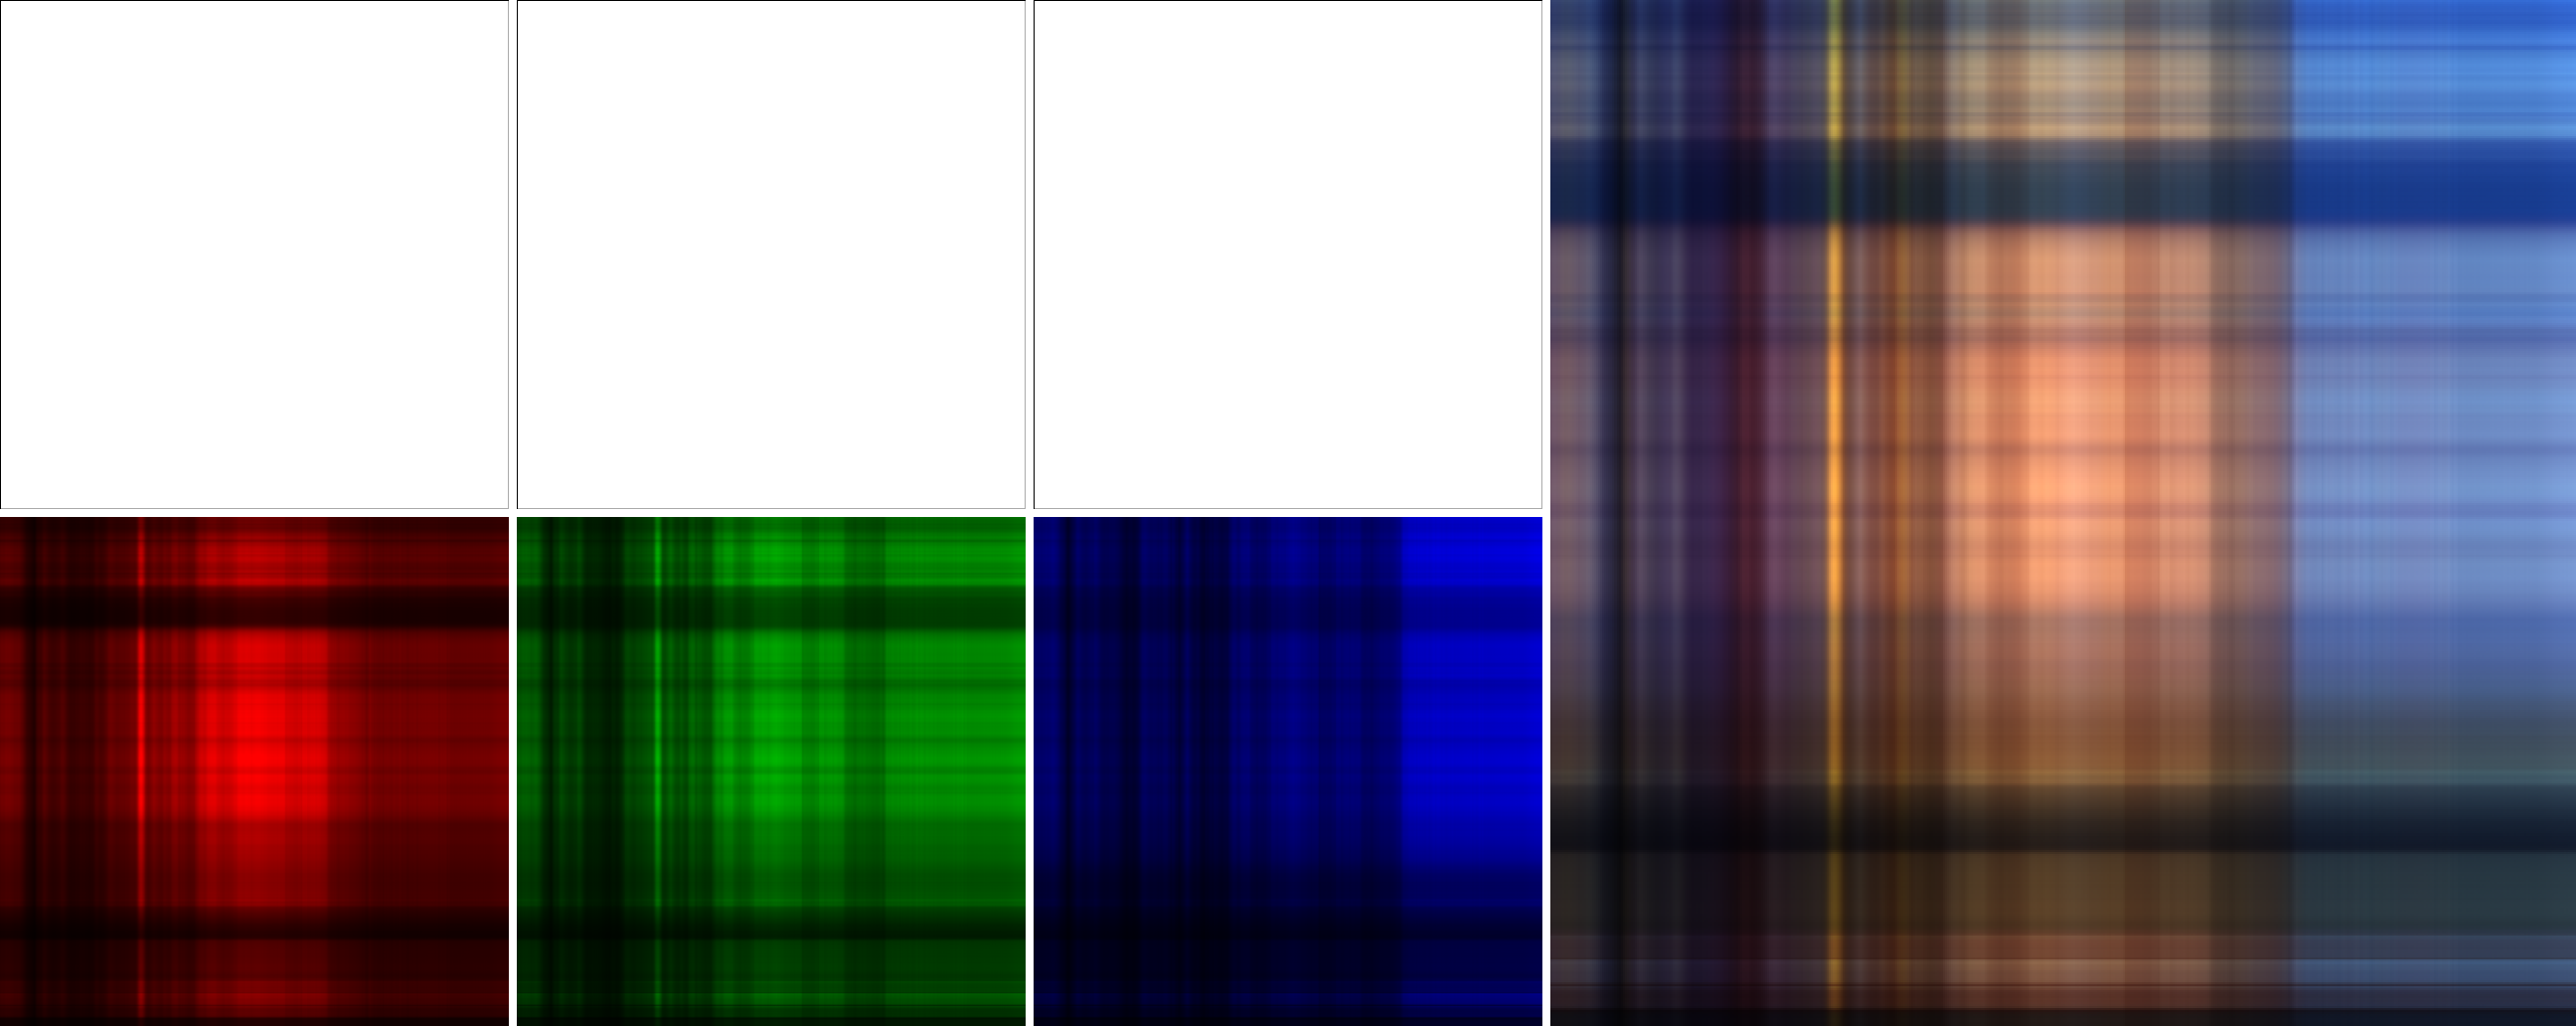
\includegraphics[width=\textwidth]{fig/r1_s1.png}
\caption{$r=1$, $\delta=\sigma_1$: macierze skompresowane R, G, B (góra), kanały R, G, B (dół) i bitmapa RGB.}
\label{fig:r1s1}
\end{figure}

\begin{figure}[H]
\centering
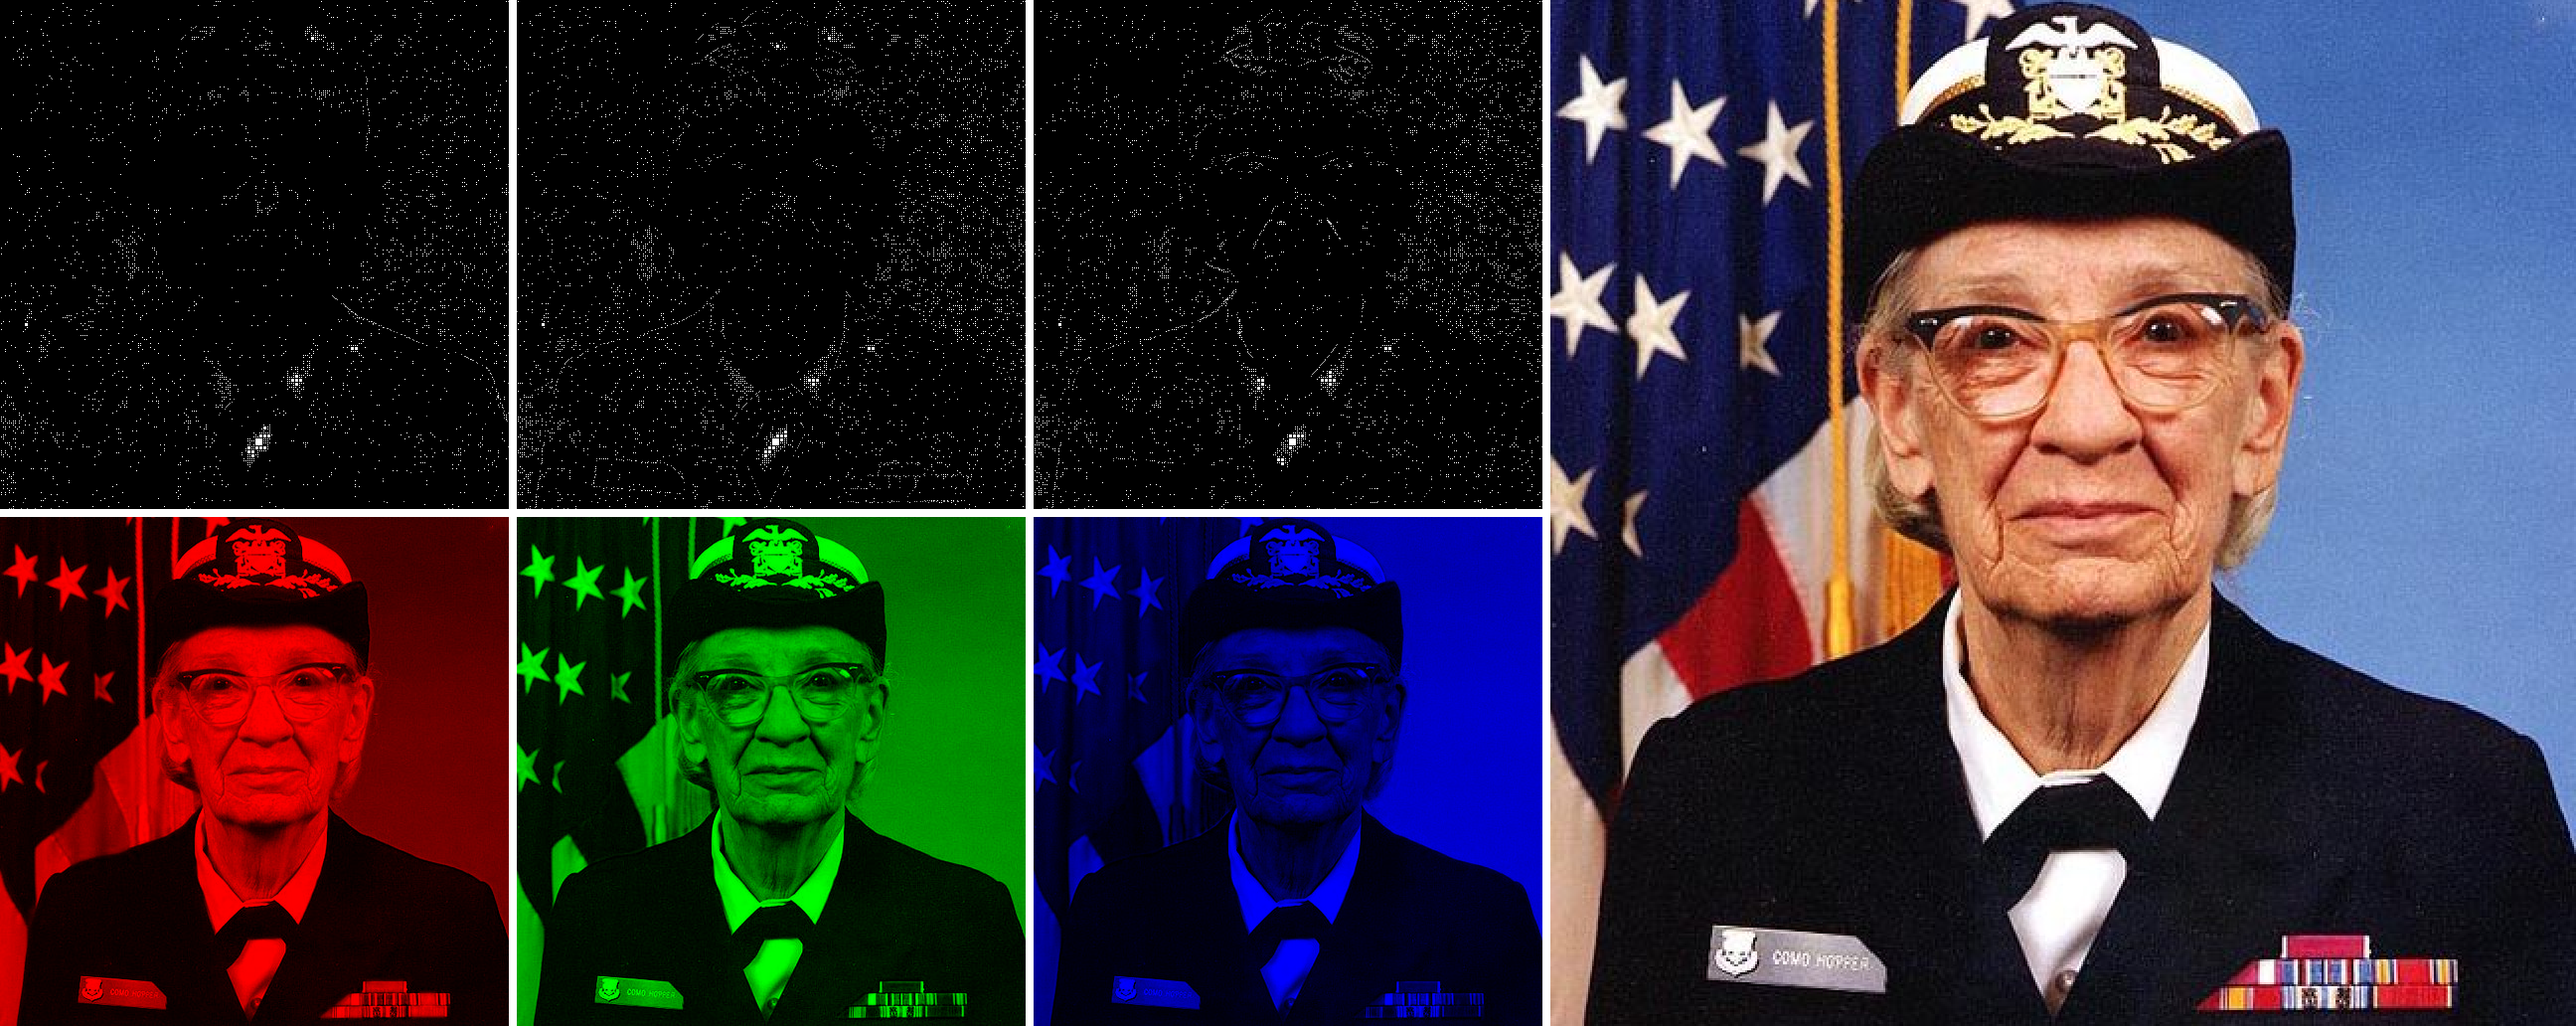
\includegraphics[width=\textwidth]{fig/r1_slast.png}
\caption{$r=1$, $\delta=\sigma_{2^k}=\sigma_{512}$: układ jak na rysunku~\ref{fig:r1s1}.}
\label{fig:r1slast}
\end{figure}

\begin{figure}[H]
\centering
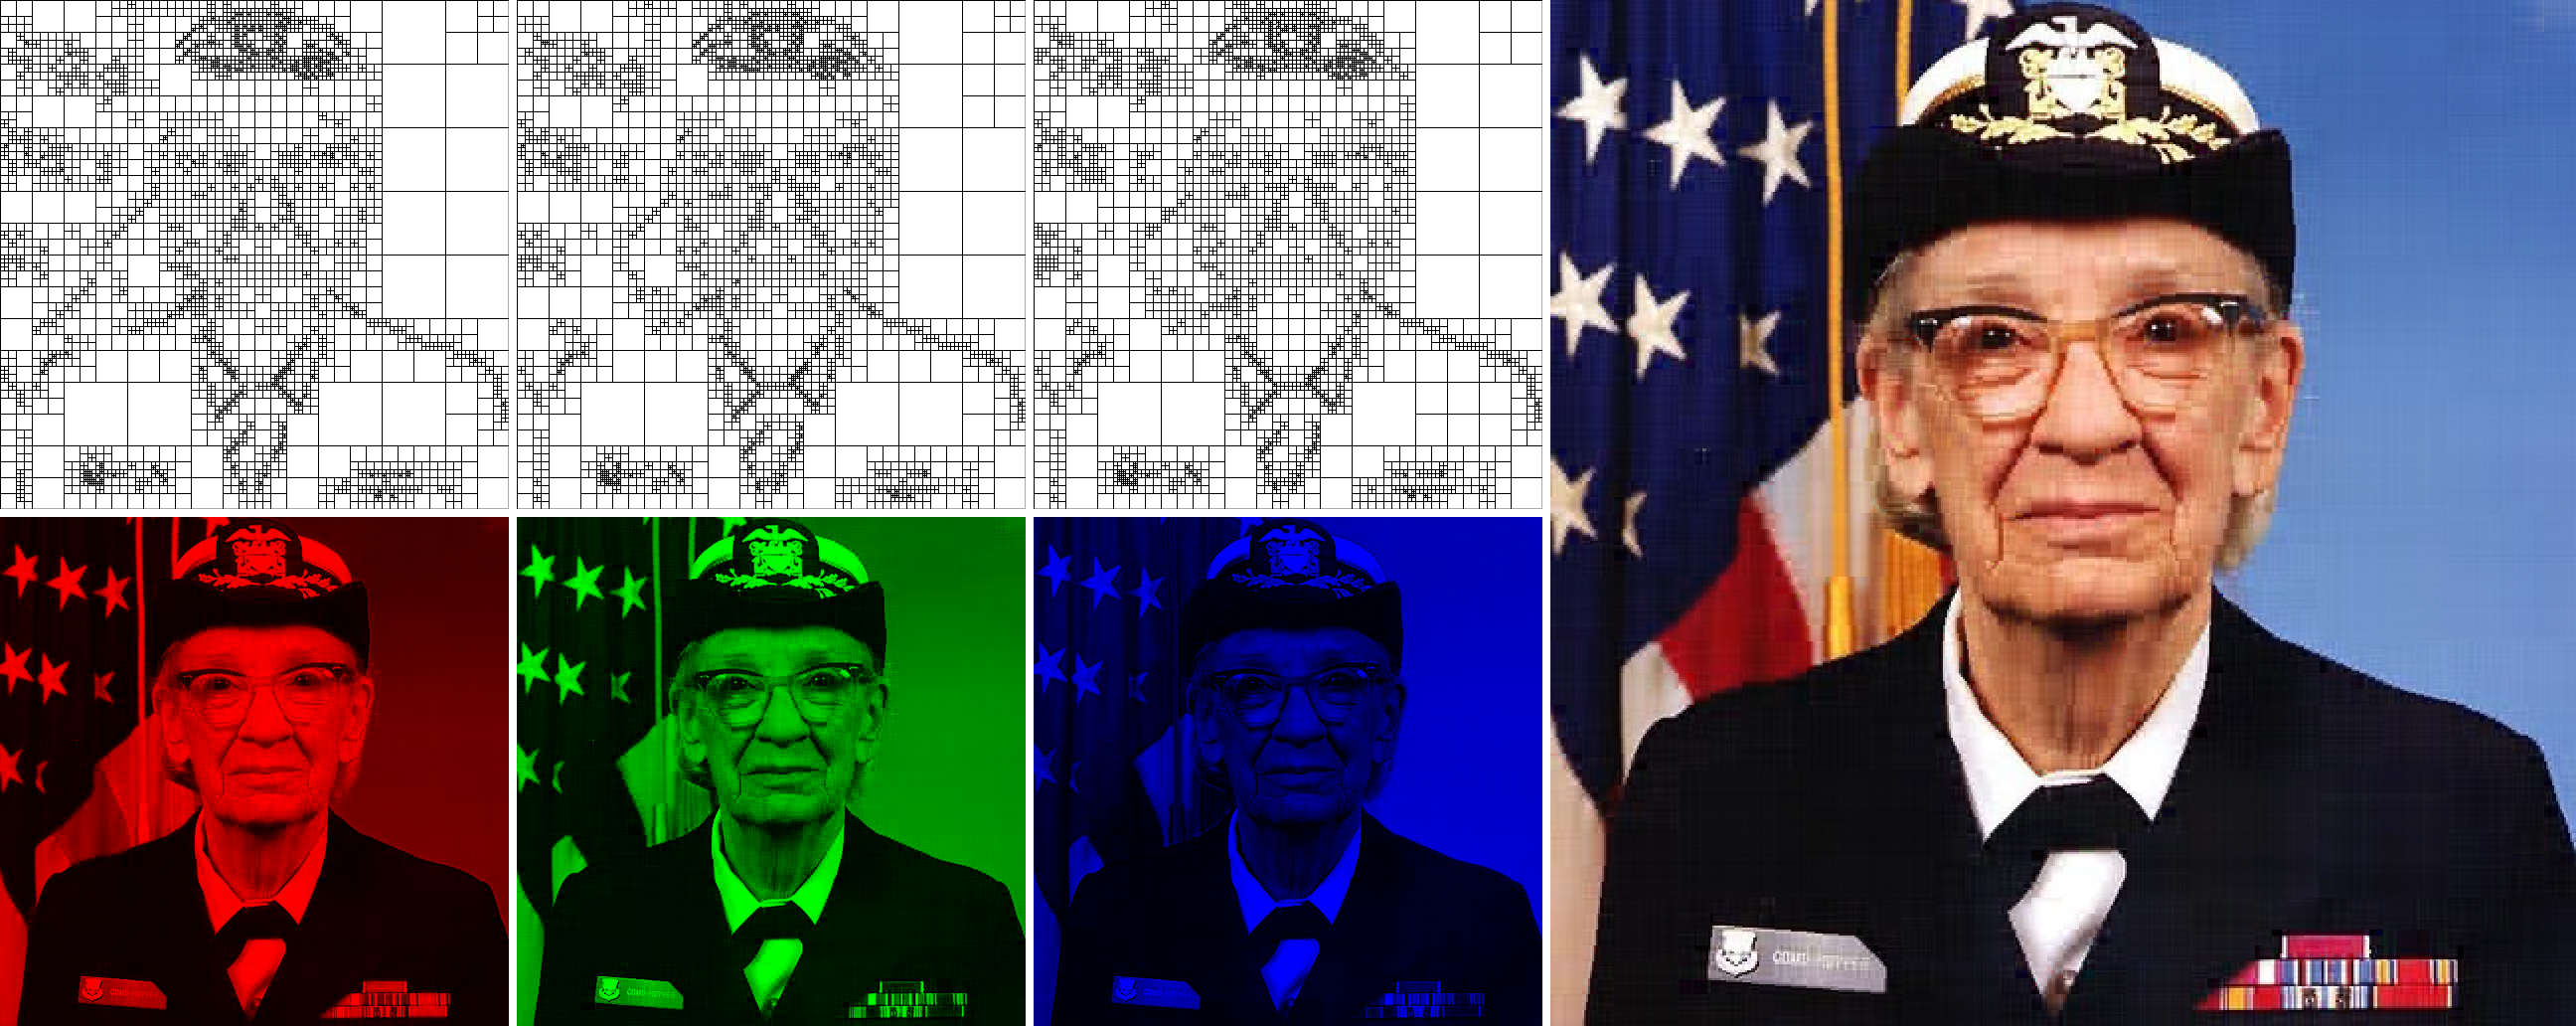
\includegraphics[width=\textwidth]{fig/r1_shalf.png}
\caption{$r=1$, $\delta=\sigma_{2^k/2}=\sigma_{256}$: układ jak na rysunku~\ref{fig:r1s1}.}
\label{fig:r1shalf}
\end{figure}

\begin{figure}[H]
\centering
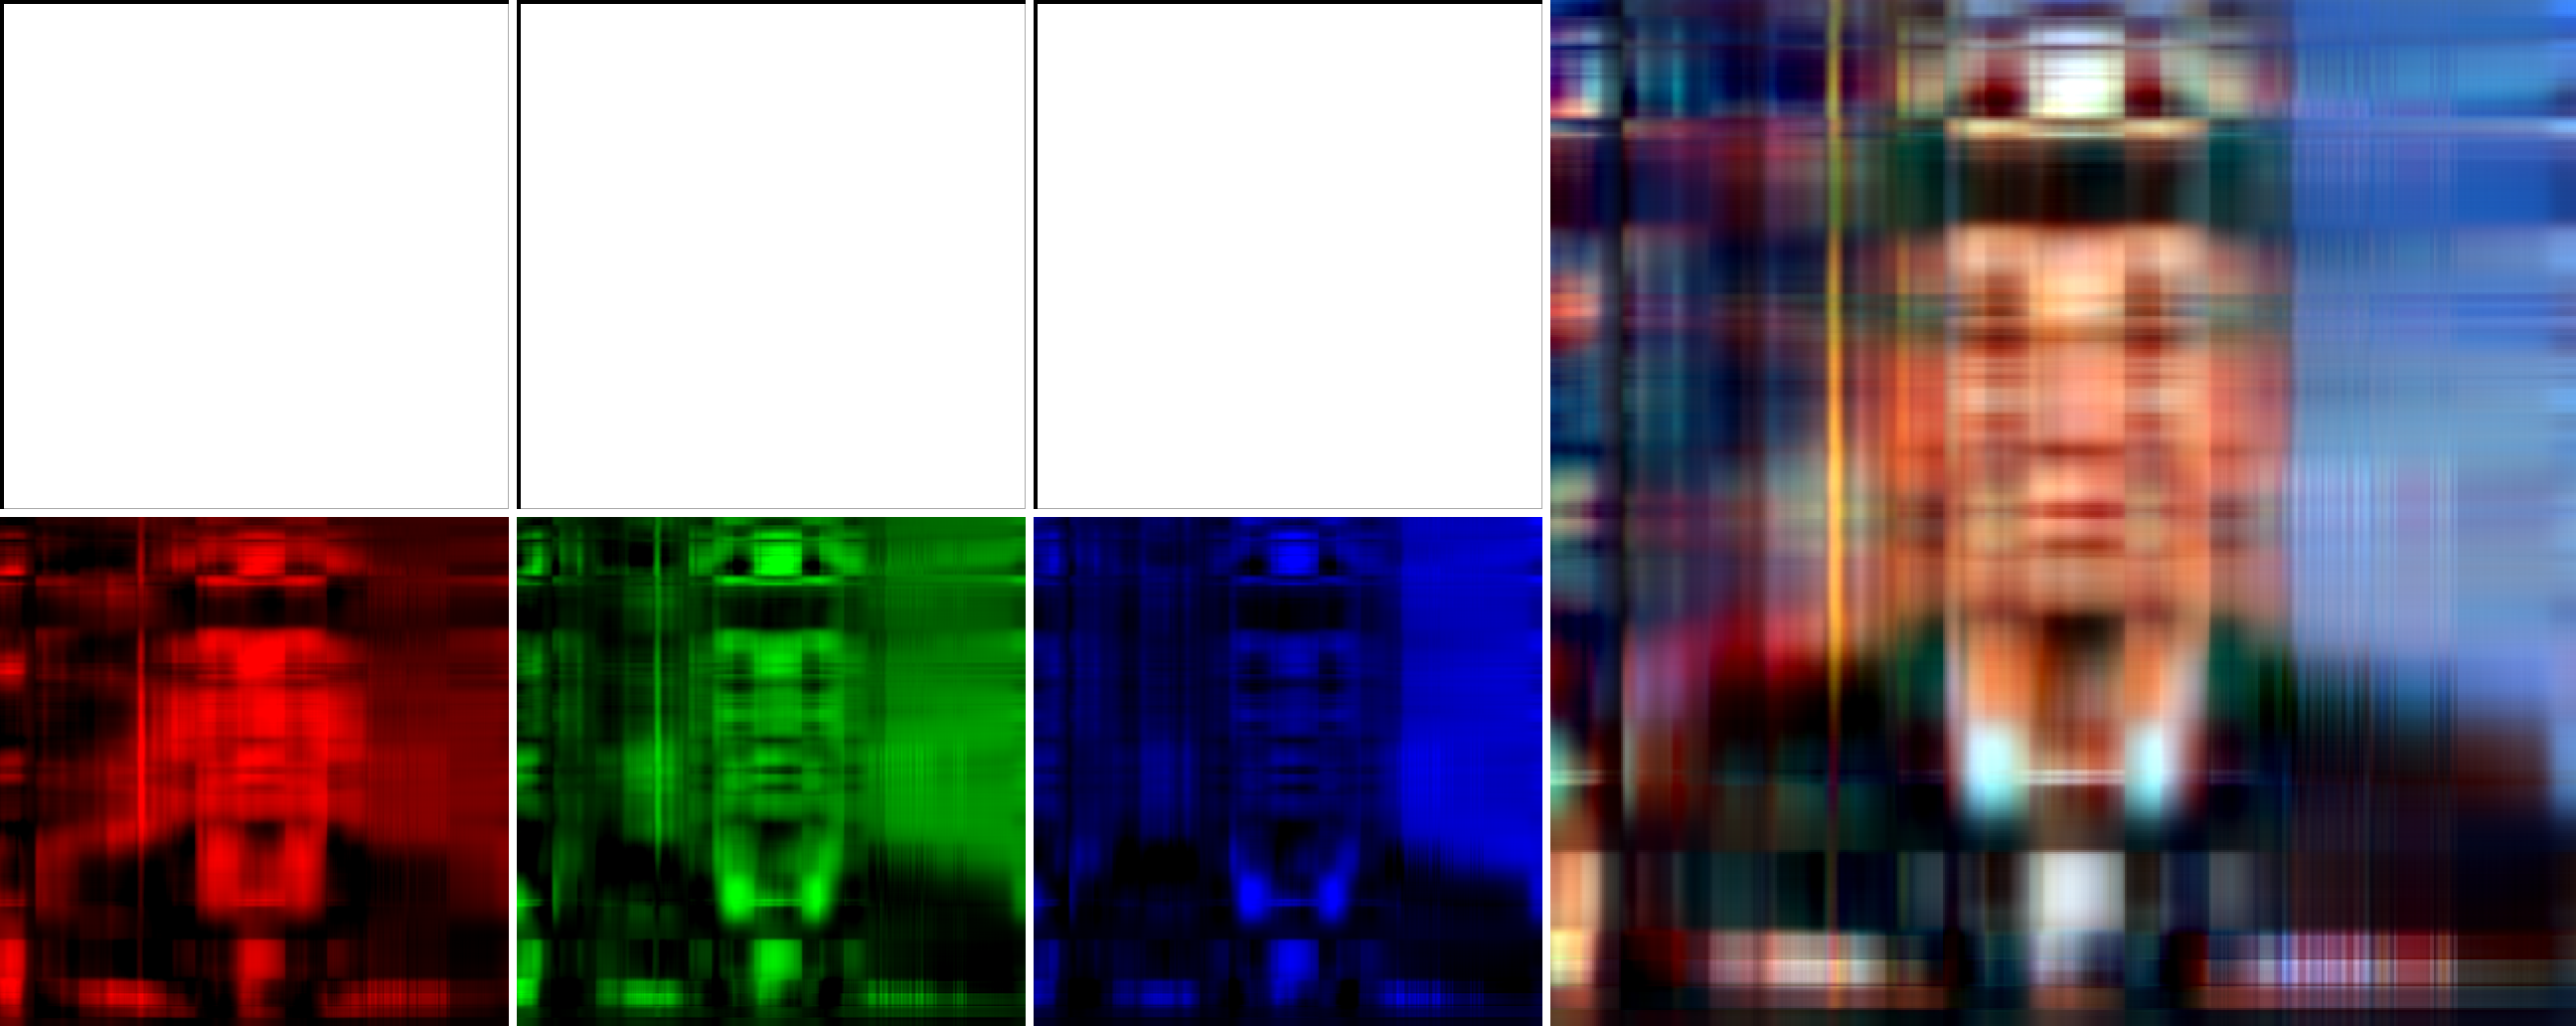
\includegraphics[width=\textwidth]{fig/r4_s1.png}
\caption{$r=4$, $\delta=\sigma_1$: układ jak na rysunku~\ref{fig:r1s1}.}
\label{fig:r4s1}
\end{figure}

\begin{figure}[H]
\centering
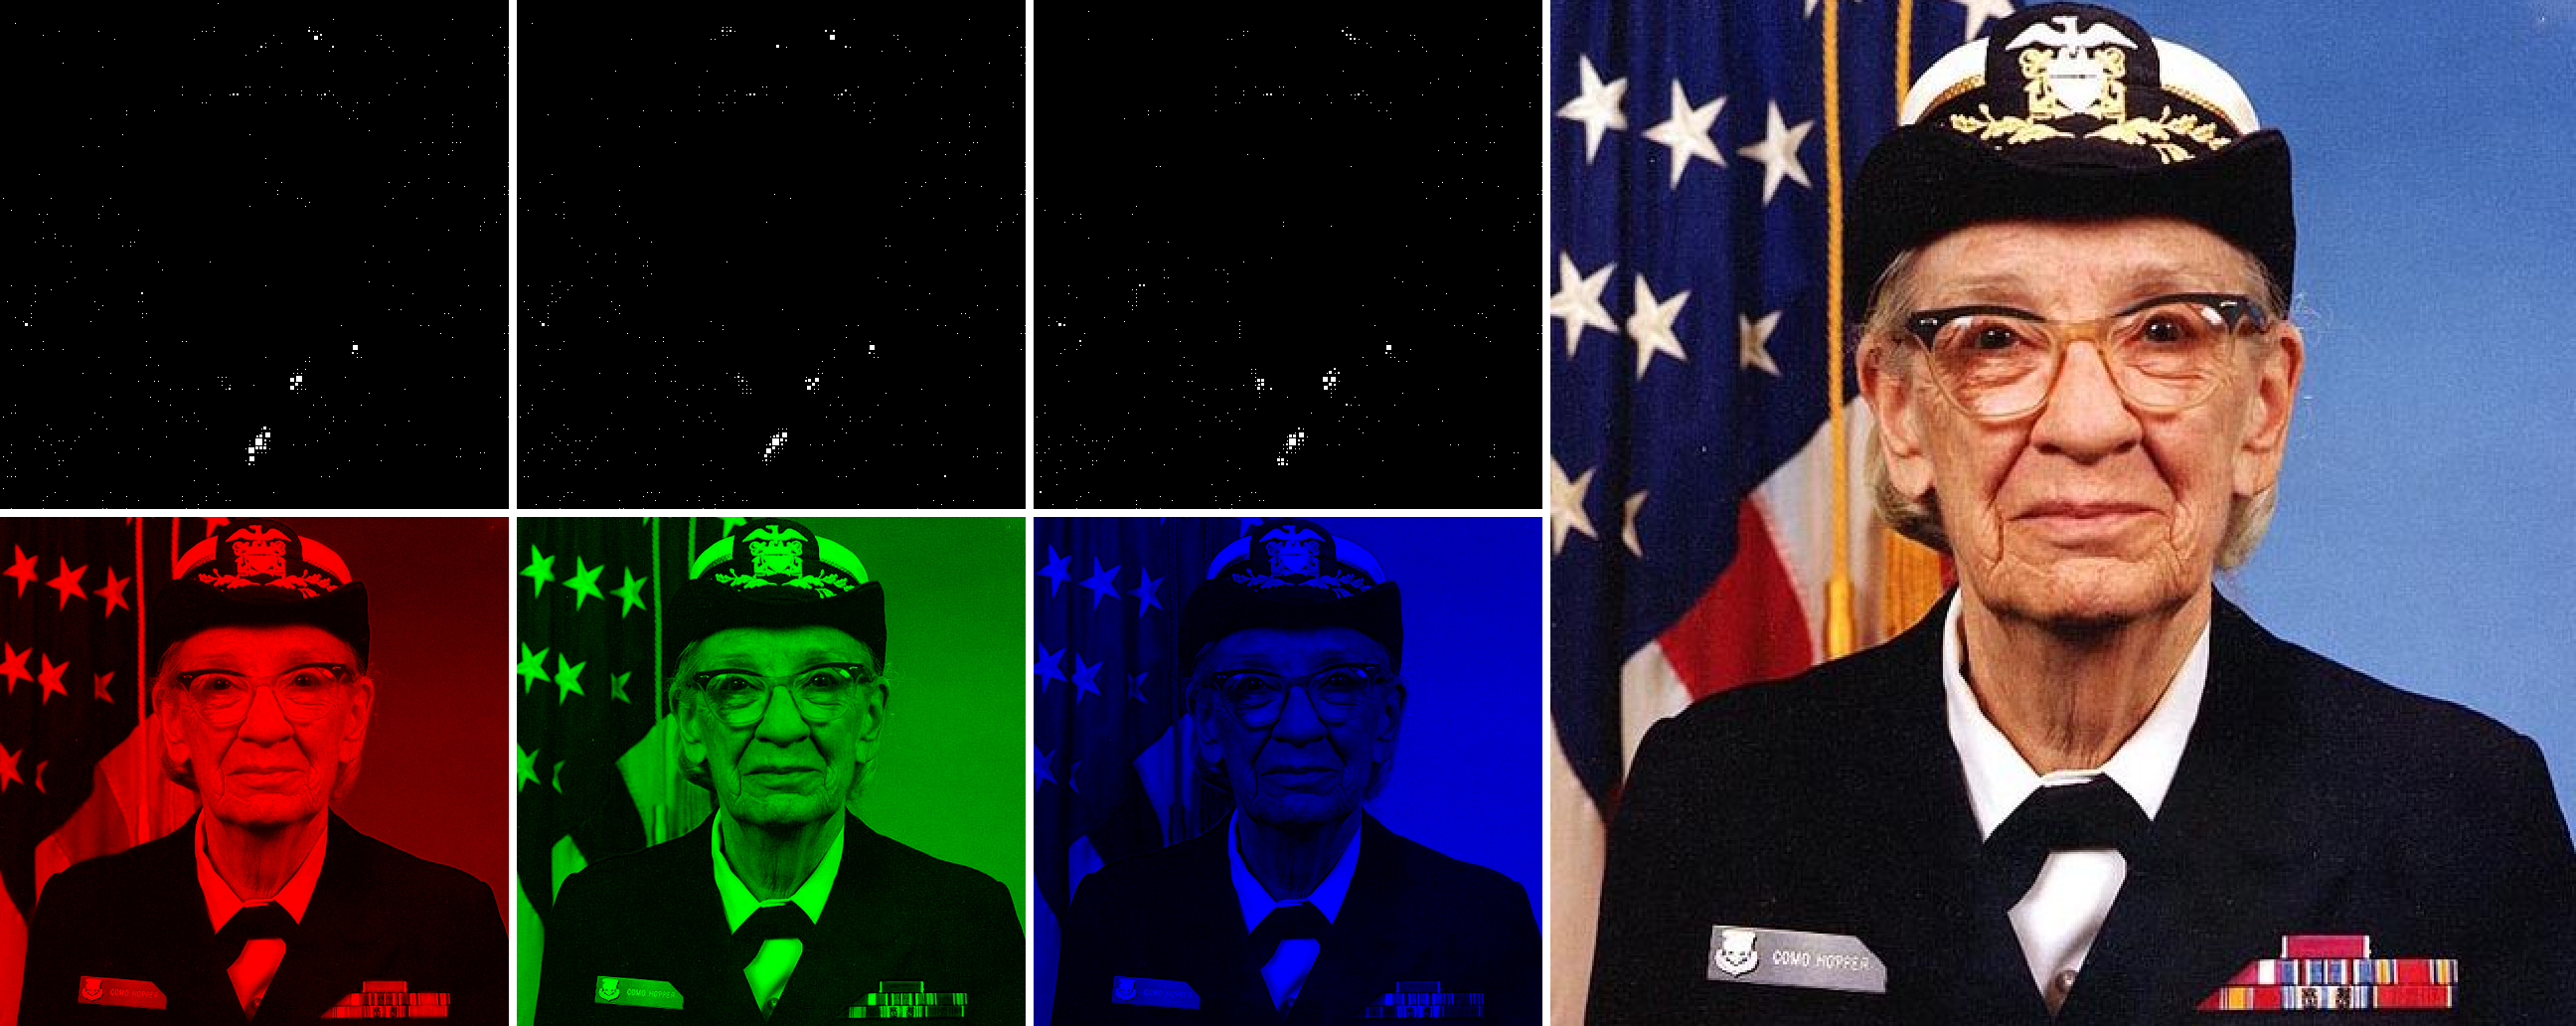
\includegraphics[width=\textwidth]{fig/r4_slast.png}
\caption{$r=4$, $\delta=\sigma_{2^k}=\sigma_{512}$: układ jak na rysunku~\ref{fig:r1s1}.}
\label{fig:r4slast}
\end{figure}

\begin{figure}[H]
\centering
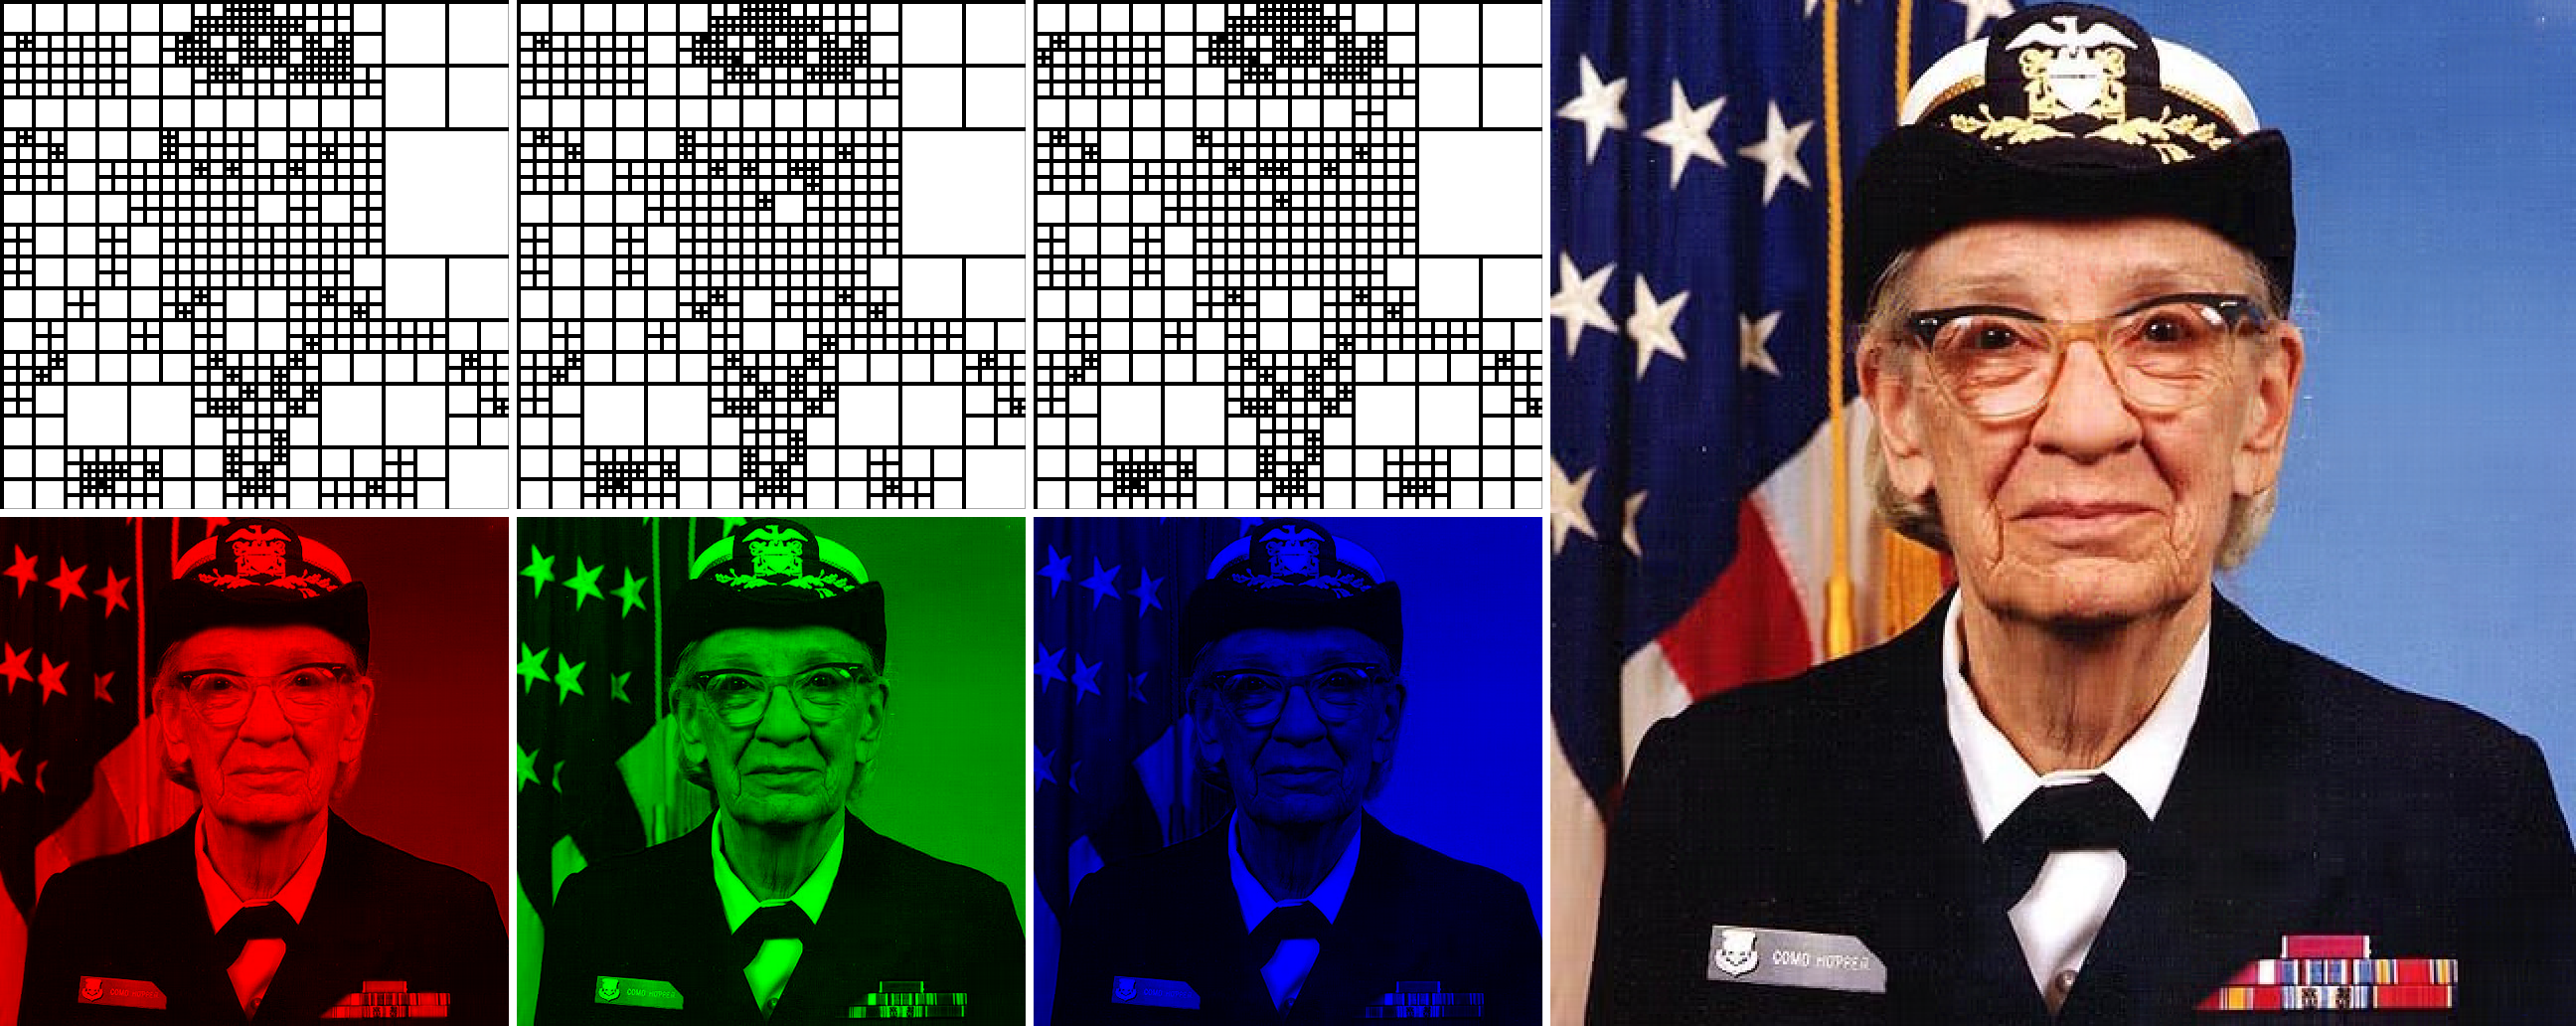
\includegraphics[width=\textwidth]{fig/r4_shalf.png}
\caption{$r=4$, $\delta=\sigma_{2^k/2}=\sigma_{256}$: układ jak na rysunku~\ref{fig:r1s1}.}
\label{fig:r4shalf}
\end{figure}

\section{Najlepsza kompresja}
Spośród wymaganych konfiguracji $\delta=\sigma_1$ daje mało pamięci i złą jakość, $\delta=\sigma_{2^k}$ bezstratny
obraz bez oszczędności pamięci, a $\delta=\sigma_{2^k/2}$ kompresję pośrednią. Żeby sprawdzić, czy da się lepiej,
przeszukaliśmy $r\in\{1,2,4,8,16\}$ i progi bezwzględne
$\delta\in\{25,50,100,200,400,800\}$ (wspólne dla trzech kanałów; odpowiadają wartościom osobliwym od około $\sigma_{60}$ do $\sigma_{390}$).
Rysunek~\ref{fig:grid} pokazuje pamięć i PSNR dla każdej pary parametrów.

\begin{figure}[H]
\centering
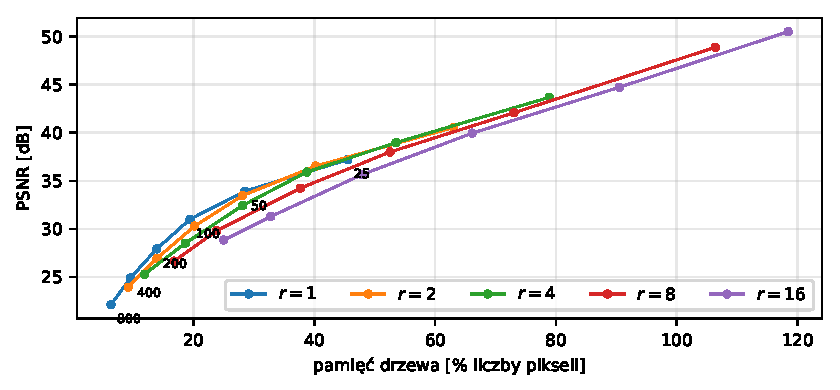
\includegraphics[width=0.72\textwidth]{fig/grid.pdf}
\caption{Pamięć drzewa i jakość bitmapy (PSNR) dla różnych $r$ i $\delta$; przy krzywej $r=1$ podano wartości
$\delta$. Wyżej i bardziej w lewo znaczy lepiej.}
\label{fig:grid}
\end{figure}

Przy tej samej pamięci najwyższy PSNR daje $r=1$: np.\ przy około 28\% pamięci $r=1$, $\delta=50$ ma 33{,}9\,dB,
$r=2$, $\delta=100$ ma 33{,}5\,dB, a $r=4$, $\delta=200$ ma 32{,}5\,dB. Niski rząd z drobniejszym podziałem lepiej
dopasowuje się do krawędzi na zdjęciu niż wyższy rząd na dużych blokach. Jako najlepszą wybraliśmy konfigurację
$r=1$, $\delta=50$: drzewo zajmuje 28{,}5\% pamięci macierzy, błąd względny kanałów wynosi 4--5\%, a PSNR 33{,}9\,dB,
przy którym różnice względem oryginału są trudne do zauważenia (rysunek~\ref{fig:best}). W porównaniu z wymaganymi
konfiguracjami daje o 3{,}3\,dB lepszą jakość niż $r=1$, $\delta=\sigma_{2^k/2}$ (za cenę 10 punktów procentowych
pamięci) oraz jakość gorszą tylko o 1{,}4\,dB niż $r=4$, $\delta=\sigma_{2^k/2}$ przy pamięci mniejszej o 8 punktów. Na rysunku macierzy widać,
że duże liście leżą w gładkich obszarach (tło, mundur), a drobne przy krawędziach (twarz, flaga, odznaczenia).

\begin{figure}[H]
\centering
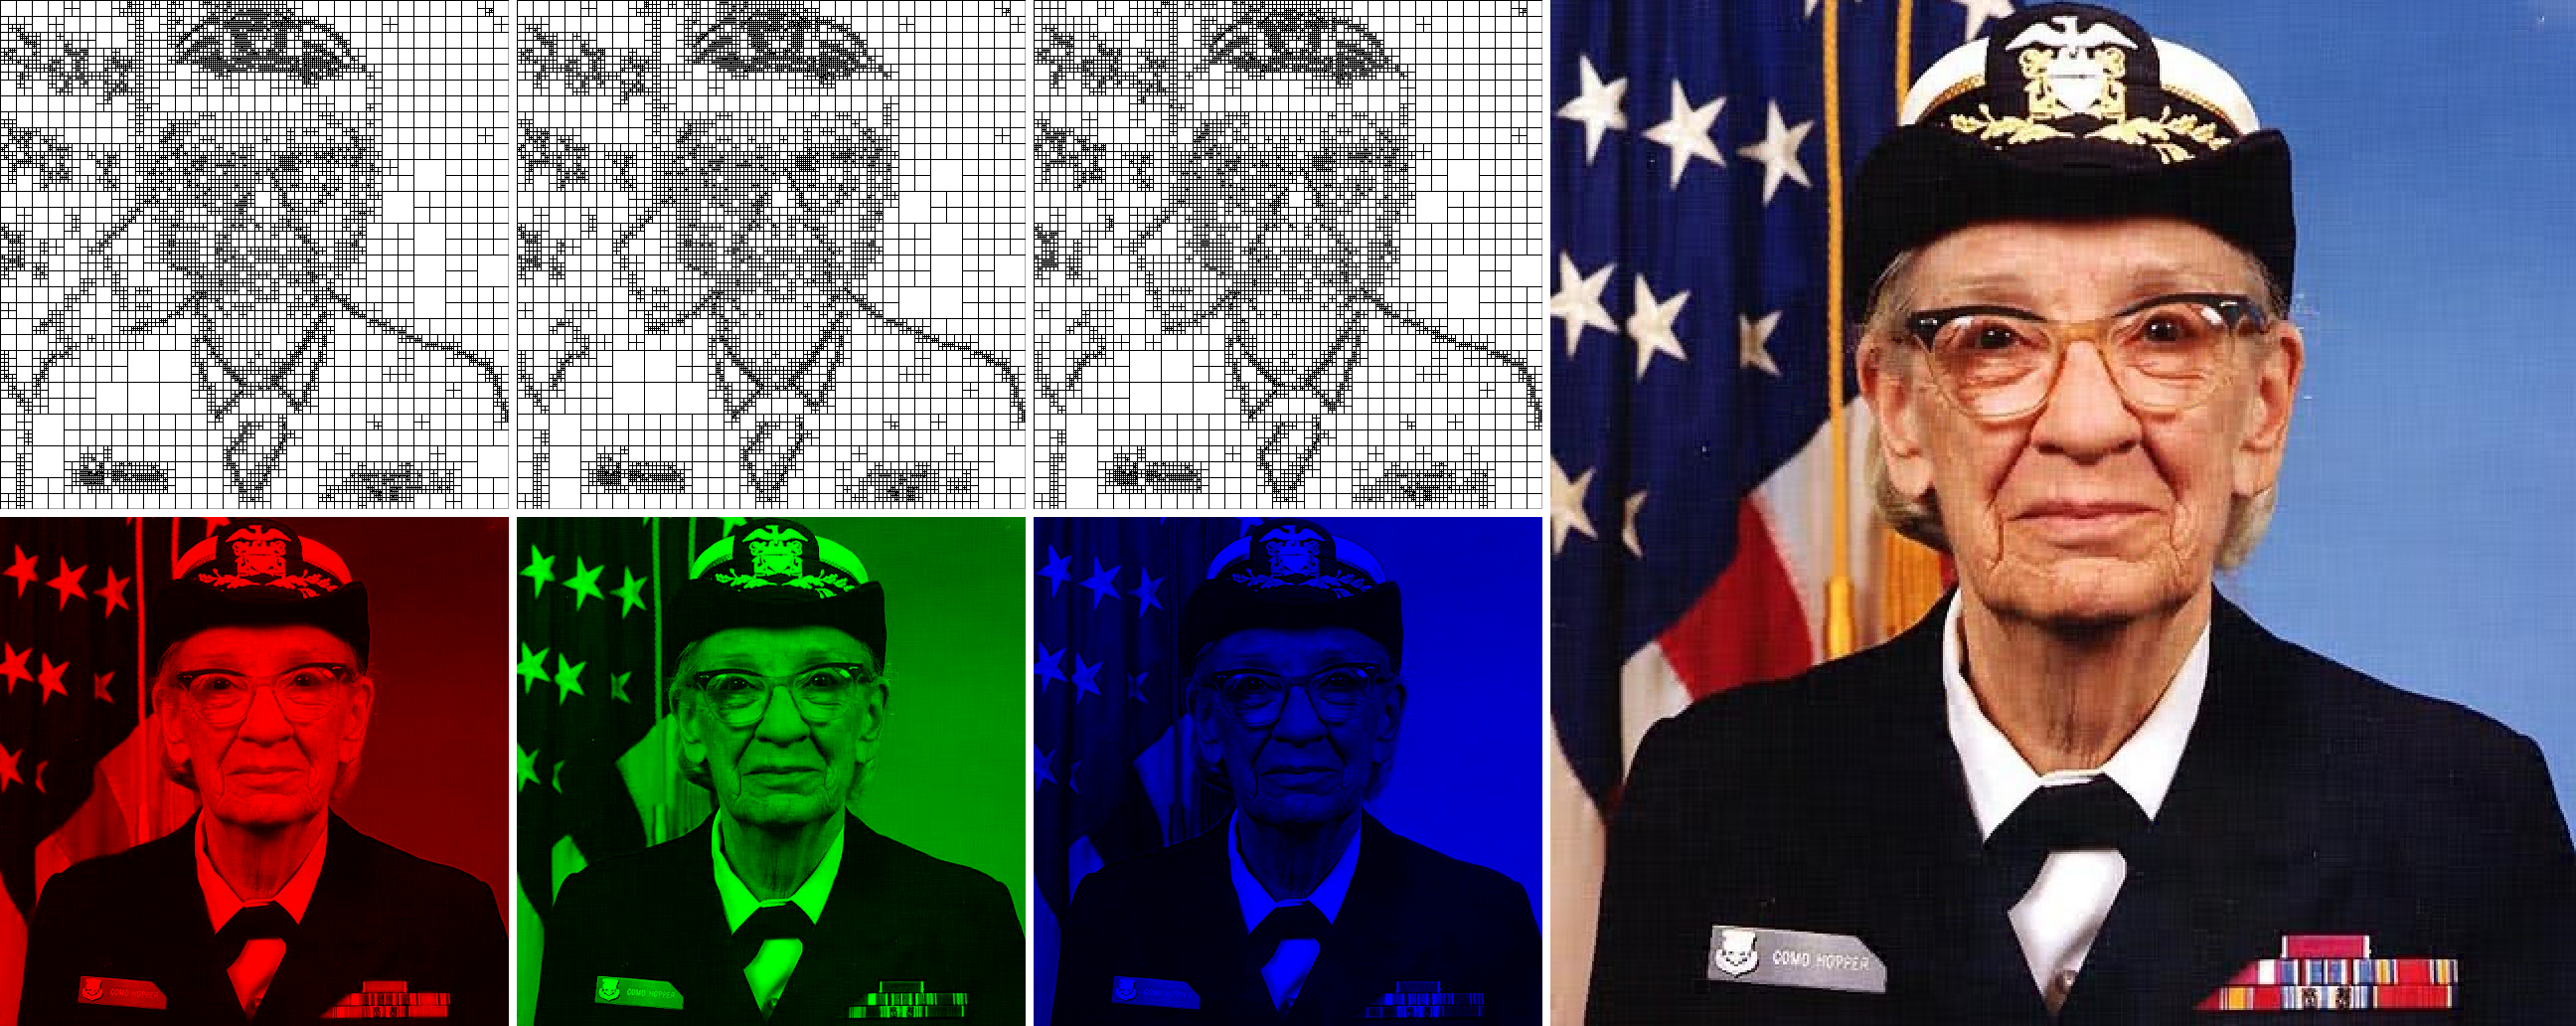
\includegraphics[width=\textwidth]{fig/best.png}
\caption{Najlepsza kompresja, $r=1$, $\delta=50$: układ jak na rysunku~\ref{fig:r1s1}.}
\label{fig:best}
\end{figure}

\section{Podsumowanie}
Kompresja dzieli bitmapę tam, gdzie obraz jest złożony, i zostawia duże bloki niskiego rzędu w obszarach gładkich.
$\delta=\sigma_1$ sprowadza macierz do jednego bloku rzędu $r$ (0{,}4--1{,}6\% pamięci, zniekształcony obraz),
$\delta=\sigma_{2^k}$ daje obraz bezstratny, ale około dwa razy większy od macierzy, a środkowa wartość osobliwa
$\delta=\sigma_{2^k/2}$ daje sensowną kompresję (18{,}5\% pamięci i 30{,}6\,dB dla $r=1$, 36{,}4\% i 35{,}3\,dB dla
$r=4$). Najlepszy znaleziony kompromis to $r=1$, $\delta=50$ (28{,}5\% pamięci, PSNR 33{,}9\,dB).

\end{document}
